\usepackage{xcolor}
\usepackage{afterpage}
\usepackage{pifont,mdframed}
\usepackage[bottom]{footmisc}
\usepackage{caption}


\createsection{\Grader}{Grader di prova}
\createsection{\Specs}{Specifiche}
\createsection{\Visualizzatore}{Visualizzatore}

\renewcommand{\inputfile}{\texttt{stdin}}
\renewcommand{\outputfile}{\texttt{stdout}}
\makeatletter
\renewcommand{\this@inputfilename}{\texttt{stdin}}
\renewcommand{\this@outputfilename}{\texttt{stdout}}
\makeatother

% % % % % % % % % % % % % % % % % % % % % % % % % % % % % % % % % % % % % % % % % % %
% % % % % % % % % % % % % % % % % % % % % % % % % % % % % % % % % % % % % % % % % % %

In occasione della XIX edizione delle Olimpiadi di Informatica, è stata avviata
la costruzione di $N$ nuovi grattacieli commemorativi a Matera, ciascuno
appaltato a un diverso costruttore. L'altezza di ciascun grattacielo verrà
decisa da Monica, in qualità di alta funzionaria delle Olimpiadi, con
l'obiettivo di costruire i grattacieli più alti senza scontentare nessuno.

In base al budget del costruttore $i$, il grattacielo $i$ può essere costruito
con una altezza massima $H[i]$. Inoltre, alcuni costruttori sono preoccupati di
sfigurare rispetto alla concorrenza, e hanno imposto dei limiti a quanto gli
altri grattacieli possano essere più alti del proprio.

Ci sono $M$ vincoli imposti dai costruttori. Ciascun vincolo $j$ è dato da tre
numeri $A_j$, $B_j$, $C_j$, e indica che il proprietario del grattacielo $A_j$
non accetta che il grattacielo $B_j$ sovrasti in altezza il suo grattacielo
$A_j$ per più di un valore $C_j$. Ovvero, indicando con $S[i]$ le altezze assegnate,
deve valere $S[B_j] \leq S[A_j] + C_j$.

Aiuta Monica a decidere le altezze di ogni grattacielo in modo da massimizzare
la \textbf{somma delle altezze} di tutti i grattacieli, rispettando le altezze
massime di ciascuno e tutti i vincoli imposti dai costruttori.

% % % % % % % % % % % % % % % % % % % % % % % % % % % % % % % % % % % % % % % % % % %
% % % % % % % % % % % % % % % % % % % % % % % % % % % % % % % % % % % % % % % % % % %

\Implementation

Dovrai sottoporre un unico file, con estensione \texttt{.cpp} o \texttt{.c}.

\begin{warning}
Tra gli allegati a questo task troverai un template \texttt{grattacieli.c} e \texttt{grattacieli.cpp} con un esempio di implementazione.
\end{warning}

Dovrai implementare la seguente funzione:

\begin{center}\begin{tabularx}{\textwidth}{|c|X|}
\hline
C  & \verb|long long costruisci(int N, int M, long long* H, int* A, int* B, int* C);|\\
C++ & \verb|long long costruisci(int N, int M, vector<long long>& H, vector<int>& A,|\\
& \hspace{4.25cm}\verb|vector<int>& B, vector<int>& C);|\\
\hline
\end{tabularx}\end{center}

\begin{itemize}[nolistsep]
	\item L'intero $N$ che rappresenta il numero di grattacieli da costruire.
	\item L'intero $M$ che rappresenta il numero di vincoli imposti dai
	      costruttori.
	\item Il vettore $H$, indicizzato da $0$ a $N-1$, che contiene le altezze
	      massime di ciascun grattacielo.
	\item I vettori $A$, $B$ e $C$, indicizzati da $0$ a $M-1$, che contengono i
	      vincoli dei costruttori.
\end{itemize}

\medskip

La funzione \texttt{costruisci} deve restituire la massima altezza totale dei
grattacieli che è possibile ottenere rispettando tutti i vincoli.

% % % % % % % % % % % % % % % % % % % % % % % % % % % % % % % % % % % % % % % % % % %
% % % % % % % % % % % % % % % % % % % % % % % % % % % % % % % % % % % % % % % % % % %

\Grader

Nella directory relativa a questo problema è presente una versione semplificata
del grader usato durante la correzione, che potete usare per testare le vostre
soluzioni in locale. Il grader di esempio legge i dati da \inputfile{}, chiama
le funzioni che dovete implementare e scrive su \outputfile{}, secondo il
seguente formato.

Il file di input è composto $M+2$ righe, contenenti:
\begin{itemize}[nolistsep,itemsep=2mm]
\item Riga $1$: gli interi $N$ e $M$.
\item Riga $2$: gli $N$ interi $H_0, \dots, H_{N-1}$.
\item Righe $3, \dots, M+2$: i tre interi $A_j$, $B_j$ e $C_j$ che rappresentano il $j$-esimo vincolo.
\end{itemize}

Il file di output consiste di una sola riga contenente il valore restituito da
\texttt{costruisci}.

% % % % % % % % % % % % % % % % % % % % % % % % % % % % % % % % % % % % % % % % % % %
% % % % % % % % % % % % % % % % % % % % % % % % % % % % % % % % % % % % % % % % % % %


\Constraints

\begin{itemize}[nolistsep, itemsep=2mm]
	\item $1 \le N, M \le 100\,000$.
	\item $1 \le H_i \le 10^{12}$.
	\item $0 \leq C_j \le 10^9$ per ogni $j$.
	\item $0 \leq A_j, B_j \leq N - 1$ per ogni $j$.
	\item Non ci sono vincoli duplicati (non esistono $j$, $k$ distinti tali che
	      $A_j = A_k$ e $B_j = B_k$).
	\item Non ci sono vincoli di un costruttore verso se stesso (tali che $A_j =
	      B_j$).
\end{itemize}

% % % % % % % % % % % % % % % % % % % % % % % % % % % % % % % % % % % % % % % % % % %
% % % % % % % % % % % % % % % % % % % % % % % % % % % % % % % % % % % % % % % % % % %


\Scoring

Il tuo programma verrà testato su diversi test case raggruppati in subtask.
Per ottenere il punteggio relativo ad un subtask, è necessario risolvere correttamente tutti i test che lo compongono.

\begin{itemize}[nolistsep,itemsep=2mm]
  \item \textbf{\makebox[2cm][l]{Subtask 1} [\phantom{1}0 punti]}: Casi d'esempio.
  % esponenziale
  \item \textbf{\makebox[2cm][l]{Subtask 2} [\phantom{1}4 punti]}: $N \leq 5$ e le altezze massime sono tutte $\leq 5$.
  % linea
  \item \textbf{\makebox[2cm][l]{Subtask 3} [\phantom{1}9 punti]}: $M = N - 1$ e $B_j = A_j + 1$ per ogni $j$.
  % DAG
  \item \textbf{\makebox[2cm][l]{Subtask 4} [\phantom{1}8 punti]}: $B_j > A_j$.
  %
  \item \textbf{\makebox[2cm][l]{Subtask 5} [21 punti]}: $N \leq 300$.
  %
  \item \textbf{\makebox[2cm][l]{Subtask 6} [16 punti]}: $C_j$ vale $0$ o $1$, per ogni $j$.
  %
  \item \textbf{\makebox[2cm][l]{Subtask 7} [24 punti]}: $N \leq 2000, M \leq 10000$.
  \item \textbf{\makebox[2cm][l]{Subtask 8} [18 punti]}: Nessuna limitazione specifica.
\end{itemize}

% % % % % % % % % % % % % % % % % % % % % % % % % % % % % % % % % % % % % % % % % % %
% % % % % % % % % % % % % % % % % % % % % % % % % % % % % % % % % % % % % % % % % % %


\Examples

\begin{example}
\exmpfile{grattacieli.input0.txt}{grattacieli.output0.txt}%
\exmpfile{grattacieli.input1.txt}{grattacieli.output1.txt}%
\end{example}

\begin{example}
\exmpfile{grattacieli.input2.txt}{grattacieli.output2.txt}%
\end{example}

% % % % % % % % % % % % % % % % % % % % % % % % % % % % % % % % % % % % % % % % % % %
% % % % % % % % % % % % % % % % % % % % % % % % % % % % % % % % % % % % % % % % % % %


\Explanation

Nel \textbf{primo caso di esempio}, ci sono 4 grattacieli e 5 vincoli.

Ecco due scelte delle altezze dei grattacieli.
In quella a sinistra, la somma delle altezze è $12$, ma non tutti i vincoli sono soddisfatti.
In quella a destra, tutti i vincoli sono soddisfatti, ma la somma delle altezze ($8$) non è massima.

\begin{center}
\hfill
\includegraphics[scale=1]{asy_grattacieli/fig1a.pdf}
\hfill
\includegraphics[scale=1]{asy_grattacieli/fig1b.pdf}
\hfill
\phantom{}
\end{center}

La massima somma delle altezze possibile è
$11$,
e si può ottenere scegliendo le altezze seguenti.

\begin{center}
\includegraphics[scale=1]{asy_grattacieli/fig1c.pdf}
\end{center}

Nel \textbf{secondo caso di esempio} la massima somma delle altezze possibile è
$16$,
e si può ottenere scegliendo le altezze seguenti.

\begin{center}
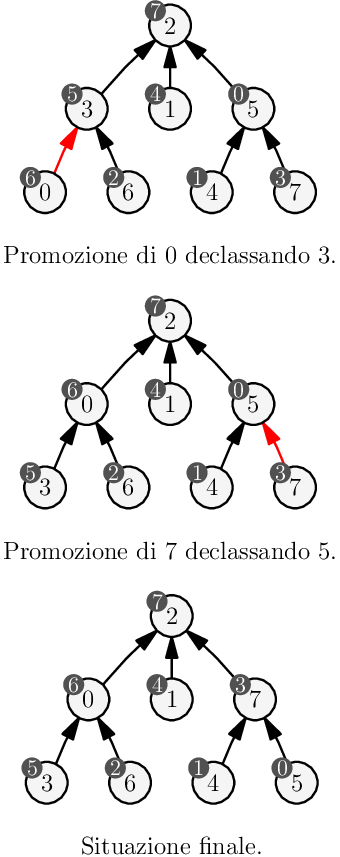
\includegraphics[scale=1]{asy_grattacieli/fig2.pdf}
\end{center}

Nel \textbf{terzo caso di esempio} la massima somma delle altezze possibile è
$54$,
e si può ottenere scegliendo le altezze seguenti.

\begin{center}
\includegraphics[scale=1]{asy_grattacieli/fig3.pdf}
\end{center}
